\documentclass[10pt]{article}

\usepackage[T1]{fontenc}
\usepackage[utf8]{inputenc}
\usepackage[margin=1in]{geometry}
\usepackage{amsmath}
\usepackage{amssymb}
\usepackage{newtxtext}
\usepackage{newtxmath}
\usepackage{microtype}
\usepackage{graphicx}
\usepackage{booktabs}
\usepackage{array}
\usepackage{tabularx}
\usepackage{rotating}
\usepackage{xurl}
\usepackage[numbers,sort&compress]{natbib}
\usepackage[colorlinks=true,linkcolor=blue,citecolor=blue,urlcolor=blue]{hyperref}

\newcolumntype{Y}{>{\raggedright\arraybackslash}X}
\setlength{\tabcolsep}{4pt}

\title{Fitting the Practice: A Data Methodology for Frontier Model Training,\\ with a Readiness Audit of 2026 Flagship Pipelines}

\author{Yugui Yu\\ YYG Strategy Lab\\ \texttt{they4897@gmail.com}}

\date{October 20, 2026 (revised)}

\begin{document}

\maketitle

\begin{abstract}
\noindent Frontier training discourse is caught between two narratives: the exhaustion of human text and the promise of fully autonomous, experience-driven learning. This paper starts from a different premise, developed in a companion theory paper (the human-referential fitting theory of AGI): the object of fitting is neither a frozen corpus nor the model's own rollouts, but human practice --- the full spectrum and full course of human experience. We specify a practice-flow data methodology as fourteen protocol components arranged across a four-layer data stack and organized into three lines: distribution as typed full-spectrum coverage (population $\times$ outcome $\times$ expertise $\times$ typicality), production as perpetual collection (production telemetry, organized failure submission, three-part failure records, domain-conditioned synthetic mixing, provenance stratification, three-tier absorption), and governance as pluralistic aggregation with institutionalized verification. Mixing ratios are domain-conditional: in verifiable domains synthetic self-sufficiency is already established, whereas open domains lack independent corrective signals, making the human practice flow an irreplaceable input there. To ground the protocol empirically, we conduct a structured disclosure audit of eight 2026 flagship pipelines against the fourteen components, scoring disclosed instantiation (0--3) with verbatim quotes. The audit yields 32/112 (mean level 0.286): typed coverage, coverage monitoring, coverage dashboards, and provenance stratification are absent from all eight disclosures; three-part failure records peak at level 1; production-line instantiation (0.393) far outruns distribution-line instantiation (0.062); and governance-line instantiation is a single-laboratory phenomenon. We close with per-component falsification conditions and translation bridges into four practitioner communities.
\end{abstract}

\medskip
\noindent\textbf{Keywords:} practice-flow data; typed experience coverage; failure-data pipeline; data readiness audit; human data injection rate

\section{Introduction}

The vocabulary of frontier-model training has shifted twice in three years. First came the wall: analyses of public human text project effective exhaustion of high-quality web corpora between 2026 and 2032 \cite{ref1}, a constraint popularized in scenario writing about compute frontiers \cite{ref2}. Then came the escape: a widely circulated essay announces a transition from ``the era of human data'' to an ``era of experience'' in which agents learn primarily from their own interaction streams \cite{ref3}. Between these two narratives sits an uncomfortable result: training recursively on model-generated data erodes distribution tails --- model collapse \cite{ref4} --- so the escape route from the wall runs through the very failure mode it was meant to avoid.

Both narratives share a hidden assumption: that ``human data'' means the \emph{stock} --- published works, scraped text, frozen snapshots of what people once wrote. A companion theory paper --- the human-referential fitting theory of AGI \cite{ref5} --- argued that this assumption is the actual error. The fitting object of a system intended to serve humans is not humanity's works but its \emph{practice}: the continuing stream of what people do, attempt, fail at, correct, and master, across the full spectrum of populations and the full course of time. The stock has a wall; the flow does not. The theory formalized this as a contrast between two fitting problems (empirical risk minimization over a fixed corpus versus online fitting of a nonstationary practice distribution), a typed coverage functional over a space of experience types, a fitting lag that behaves like regret in nonstationary online learning, and four boundary conditions on what may be fitted, by whom, under which institutional constraints, and how self-reference is contained. A prior empirical audit \cite{ref6} established the companion fact on the failure side of the stock: failure data is treated as exhaust. Of 33 surveyed training-data lifecycle artifacts, none gave failure records first-class status (0/33); mainstream recipes contained essentially no structured failure treatment (0/15 at level 3 or above on a five-level scale, versus 4/5 for five flagship agentic pipelines); and no public dataset packages error type, root cause, and corrective replay together.

What is missing between the theory and the audit is the middle layer: an \emph{engineering methodology}. The theory says what should be fitted; the audit says what current practice does with one slice of the stock. Neither specifies the pipeline --- the components, interfaces, and institutional arrangements --- that would make practice itself a trainable data supply. Nor does the existing literature: distribution-side research matured into output-diversity engineering \cite{ref7}, production-side engineering matured into scattered flywheel practice \cite{ref8}, and governance-side research matured into licensing and provenance studies \cite{ref9,ref10}, but no prior work gives a pipeline-level protocol for fitting the human practice flow, and no prior work audits flagship pipelines against such a protocol. Engineering talk of ``data flywheels'' predates this paper and circulates widely; what it lacks is exactly what a methodology must supply --- typed coverage targets, failure-record specifications, domain-conditioned mixing rules, and institutional verification, in one coherent protocol.

This paper supplies that middle layer and then measures the distance between it and current flagship practice. Its contributions are fourfold:

\begin{enumerate}
\item \textbf{A fourteen-component protocol specification} (C1--C14), organized as three methodology lines --- distribution, production, governance --- across a four-layer data stack (Section 2; Sections 3--5). Each component is given an operational definition, a protocol specification, failure modes, and a clearly separated summary of existing instantiation.
\item \textbf{A readiness audit} --- the paper's original instrument: the fourteen components are scored against the public disclosures of eight 2026 flagship pipelines (5 technical-report-grade, 3 system-card/announcement-grade), yielding a $8\times14$ matrix of \emph{disclosed instantiation} levels, with verbatim quotes and locators for every non-zero cell (Section 6, Tables 1--4, Figure 2).
\item \textbf{A domain-conditioned theory of synthetic mixing}, in which the required rate of human-flow injection is a per-domain design parameter: verifiable domains admit synthetic self-sufficiency on a human-pretrained base, while open domains --- values, experience coverage, long-tail practice --- provide no independent corrective signal, so the human practice flow is irreplaceable there (Section 4.5).
\item \textbf{Translation bridges and falsification conditions}: four discourse bridges that carry the methodology into the agent-RL, data-engineering, governance, and philosophical communities respectively (Section 7), and per-line falsification conditions under which the methodology would be refuted or demoted (Section 8).
\end{enumerate}

A note on epistemic status, because this paper deliberately mixes two registers. Sections 3--5 are \emph{normative}: they specify what a practice-fitting pipeline should and must do, and their warrant is theory plus literature, not observed practice. Section 6 is \emph{descriptive}: it reports what flagship pipelines disclose, with a construct --- disclosed instantiation --- that measures documentation, not implementation (``not disclosed'' never means ``not implemented''). The audit is never used to prove the protocol correct, and the protocol never masquerades as a description of practice. Section 9 returns to the temporal clause that motivates everything: a stock can be bought, walled, and exhausted; a flow must be collected, typed, cleaned, absorbed, and governed --- continuously.

\section{The Data Stack of Practice-Fitting}

Figure~\ref{fig:stack} gives the architecture. The stack has four layers. A \textbf{collection layer} acquires raw practice: production telemetry (C5), organized failure submission (C6), and real task libraries that feed typed collection (C1, C3). A \textbf{cleaning layer} turns raw acquisition into trainable records: pseudo-failure discrimination and environment sanitization (C8), three-part failure records (C7), provenance stratification (C10), and domain-conditioned mixing (C9). An \textbf{absorption layer} moves cleaned records into the model on three clocks: continued pre-training (CPT) cadence, offline reinforcement-learning (RL) replay, and runtime memory, with an explicit division of labor (C11). A \textbf{governance band} spans all stages: coverage monitoring and dashboards (C2, C4) make the distribution auditable, while pluralistic aggregation (C12), verifier institutionalization (C13), and consent-based feasible-set management (C14) decide whose practice is fitted, who adjudicates failures, and which data is permitted to enter at all.

\begin{figure}[t]
\centering
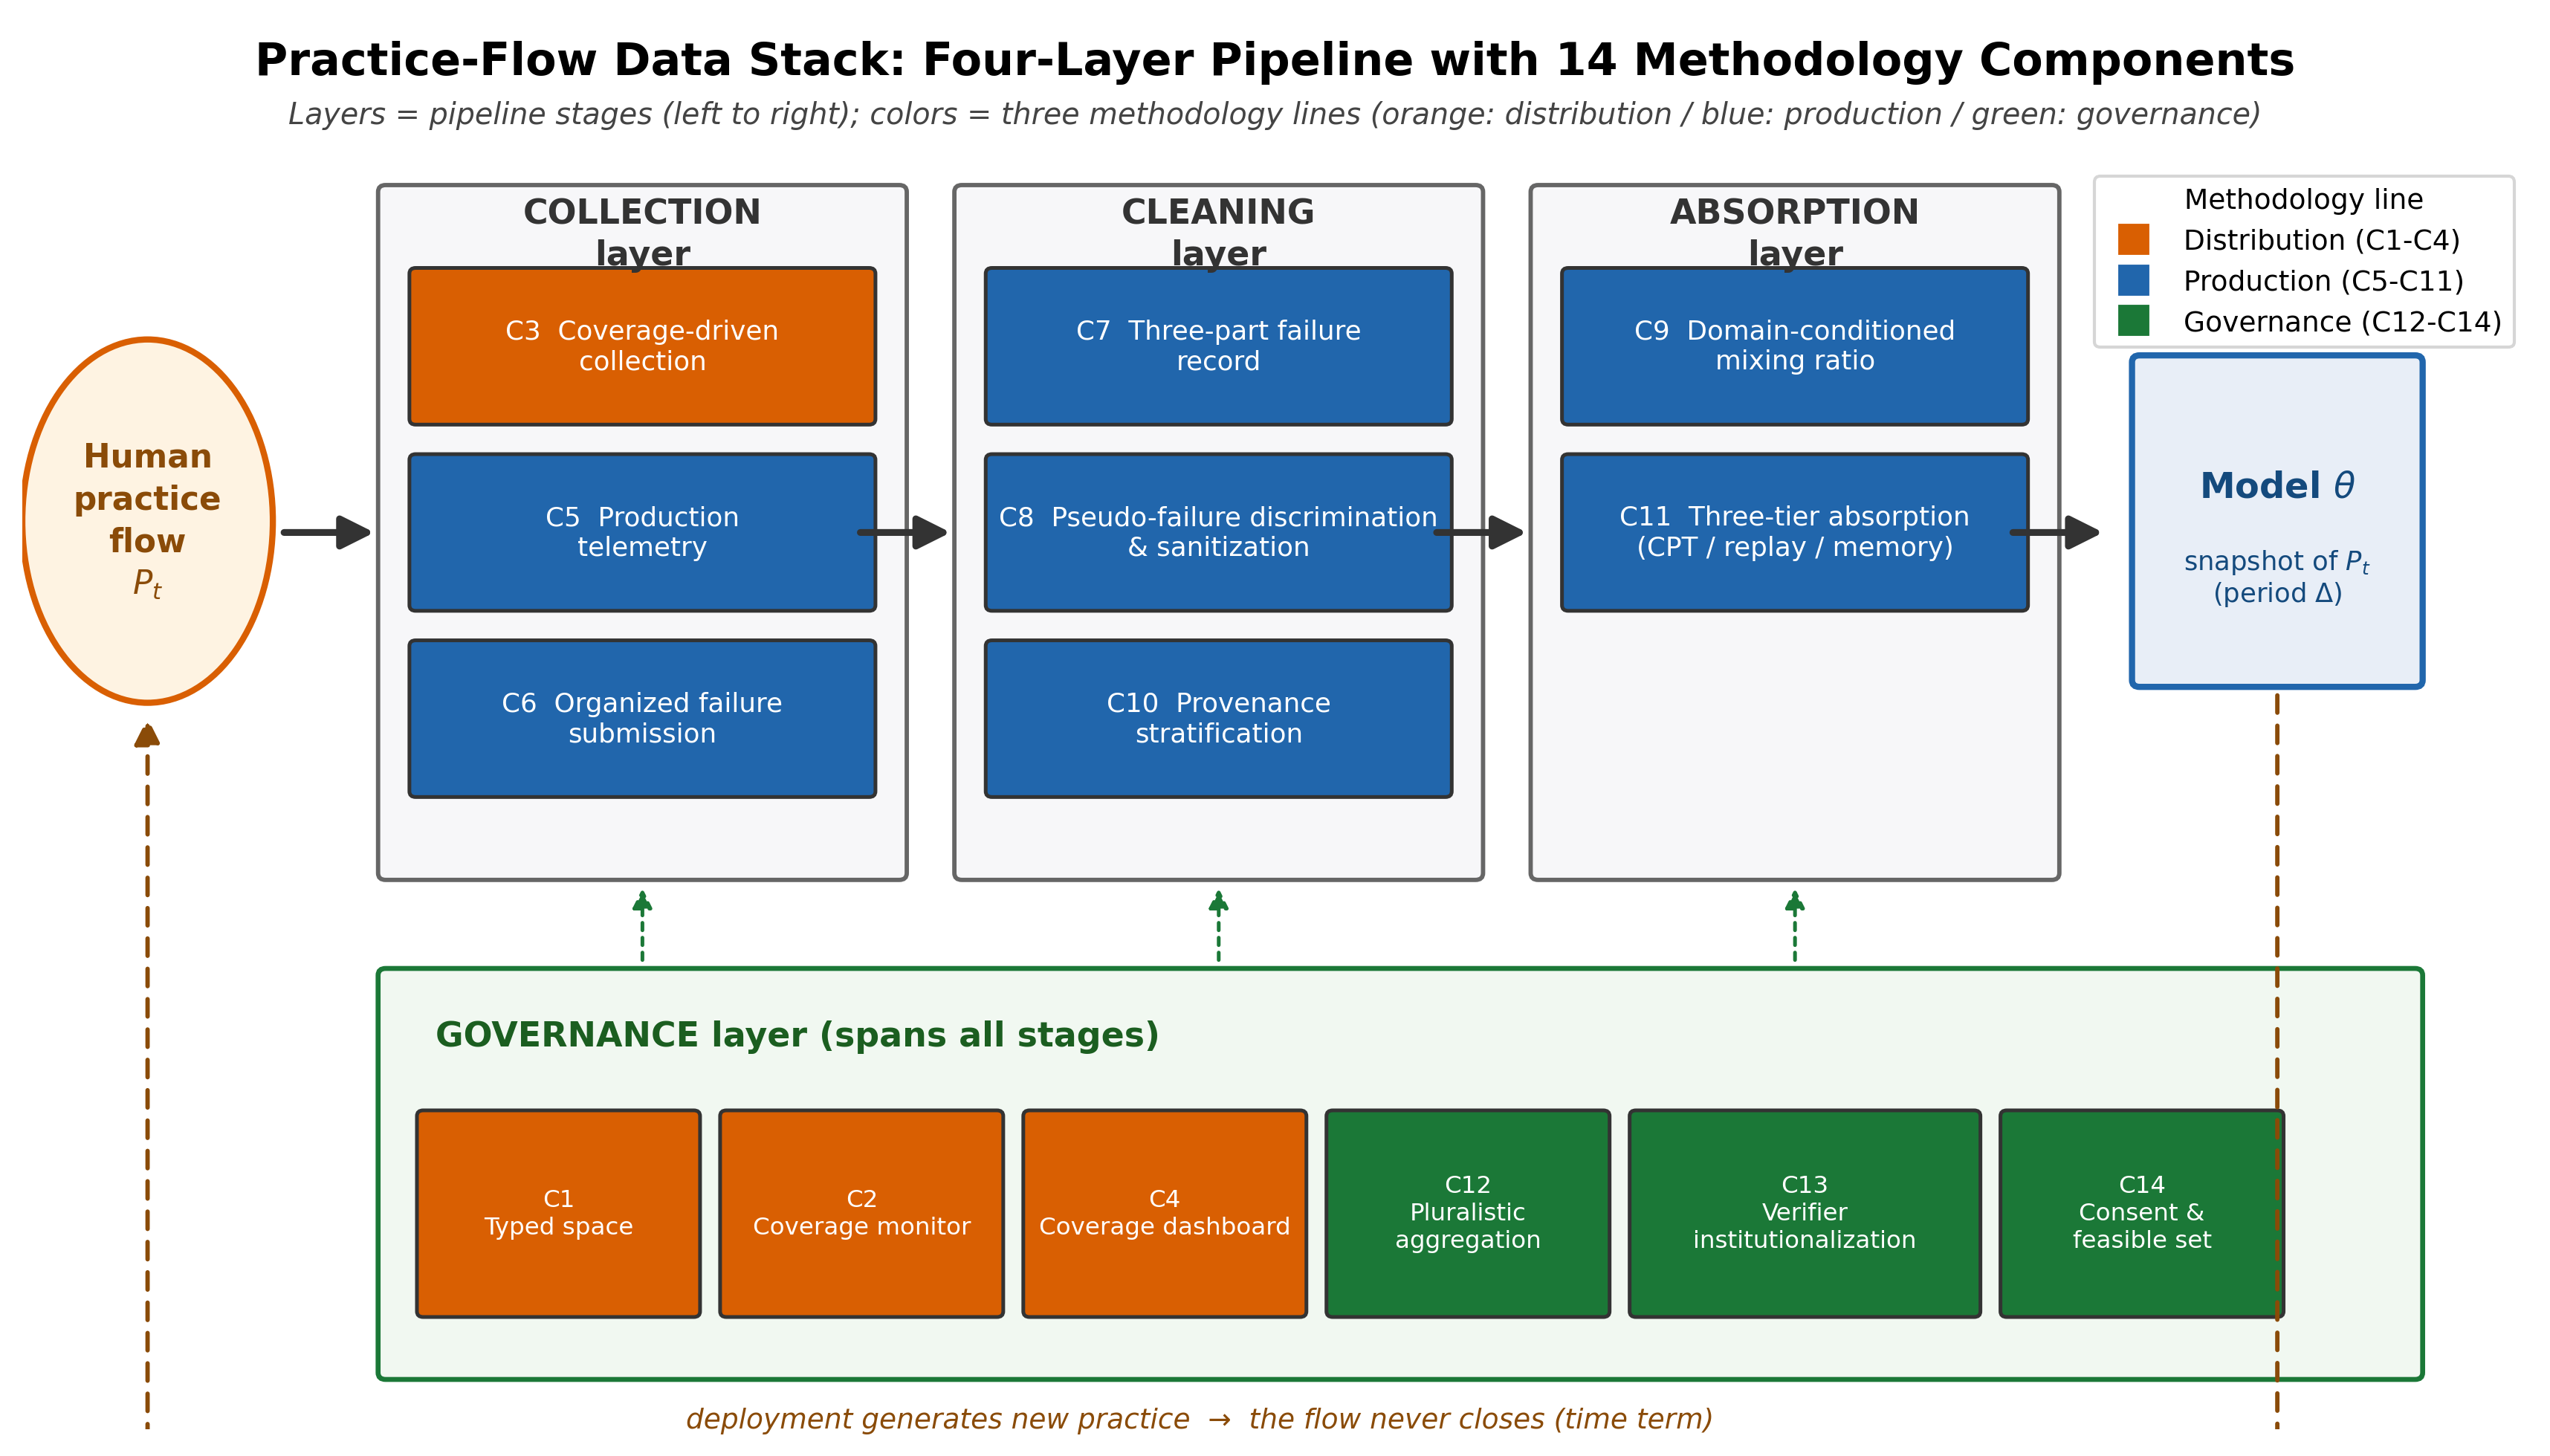
\includegraphics[width=\textwidth]{figures/fig1_data_stack_architecture.png}
\caption{The practice-flow data stack. Four pipeline layers (collection $\to$ cleaning $\to$ absorption, with a governance band spanning all stages) hosting the 14 methodology components (C1--C14). Box colors encode the three methodology lines (orange = distribution, blue = production, green = governance); the dashed loop marks the never-closing flow of human practice (the time term).}
\label{fig:stack}
\end{figure}

Two organizational cuts cross-cut the figure. By \emph{line}: C1--C4 form the distribution line (what to collect --- the typed full spectrum), C5--C11 the production line (how to collect, clean, and absorb it in perpetuity), and C12--C14 the governance line (who decides and verifies). By \emph{function}: C1, C2, C9, C10, and C11 are measurement-heavy components that make the flow computable; C3, C5--C8 are acquisition- and cleaning-heavy; C12--C14 are institution-heavy. The mapping to the companion theory is direct and stated once per component in Sections 3--5: C1--C4 operationalize the typed coverage functional; C9 exists because of collapse results and the self-reference boundary; C11 exists because the fitting lag is a regret term; C14 exists because the institutional boundary is a dynamic feasible set, not a one-time check.

Three design rules govern every component specification that follows. First, \emph{operational definitions must be coder-independent}: two readers of the same document, applying the definition, reach the same verdict --- this is what makes the audit in Section 6 possible at all. Second, \emph{every component separates the protocol (should/must) from existing instantiation (is)}: each component ends with an explicitly marked instantiation paragraph that cites only verifiable public practice. Third, \emph{every component carries its own failure modes and falsification condition}: a methodology that cannot say how it would break is a slogan, not a protocol (Section 8 tabulates these).

\section{Distribution = Full-Spectrum Coverage}

\subsection{Typed space definition (C1)}

\emph{Operational definition.} The corpus is assigned a four-dimensional type schema $\tau$ = population $\times$ outcome $\times$ expertise $\times$ typicality, with frozen value sets and executable labeling rules for every dimension. \emph{Protocol.} Outcome $\in$ \{success, failure, mixed\} is labeled from the trajectory record itself. Expertise is graded on observable proxies --- revision counts under review, years in role, task-specific acceptance history --- never on self-report alone. Typicality is the frequency quantile of the cell the sample falls in, estimated against a reference distribution declared in advance. Population classifies \emph{whose} practice (practitioner, affected party, evaluator). Each dimension ships with a labeling guide and two calibration examples; a pilot of 100 labels per dimension must reach 80\% agreement before full annotation begins, and the frozen schema is versioned like code. \emph{Why this component.} The coverage functional of the companion theory integrates over a typed space; a diversity rhetoric without a schema computes nothing. In the companion audit of 80 training-objective specifications, an operator resembling typed experience coverage appeared zero times \cite{ref5}. A caveat fixed here in wording: the phrase ``experience coverage'' has begun circulating in 2026 --- in work on solution-mode collapse in RL with verifiable rewards, where it refers to the diversity of the model's \emph{own correct solutions} \cite{ref11}, and in a non-peer-reviewed position paper on recursive self-improving agents, where it refers to the width of an \emph{agent's} experience \cite{ref12}. The term has begun circulating; its operationalization as a typed \emph{data} coverage axis remains absent --- both uses sit on the output or agent side, not on the design of training-data distributions. \emph{Failure modes.} Unobservable proxies (an ``expertise'' grade with no behavioral trace), label noise, and coupled dimensions masquerading as independent coverage. \emph{Existing instantiation.} None located on the data side; the nearest neighbors are output-distribution taxonomies (Spectrum Suite's task $\times$ data-source organization \cite{ref7}) and solution-mode typing in RLVR dynamics \cite{ref11} --- neither types a \emph{corpus} of human practice.

\subsection{Coverage monitor (C2)}

\emph{Operational definition.} A reproducible program that samples the training-data distribution, estimates per-cell frequencies with uncertainty, reports cell coverage, and raises an alarm when the smallest cells vanish. \emph{Protocol.} Periodic samples (e.g., $n \ge 10{,}000$ weekly) are typed under C1's schema; cell frequencies are estimated with Wilson intervals; the reported statistic is $\Sigma\,\min(\hat{q},\hat{p})$ over cells --- a directly computable surrogate for the theory's overlap functional --- alongside the count of empty cells. Alarms fire when a cell count falls below a floor or drops more than 50\% period-over-period, and each alarm becomes a work item, not a log line. The reference distribution must be \emph{external lineage} (historical corpus, task-source census), never the model's own output, or the monitor degenerates into self-confirmation. \emph{Why.} The practice distribution is not directly observable; overlap with it can only be estimated by sampling, and mode collapse --- the mechanism formalized as tail loss \cite{ref4} --- appears first in the smallest cells. \emph{Failure modes.} Self-referential baselines, noisy sparse cells, and dimensionality that makes every cell sparse (the schema must stay coarse enough to fill). \emph{Existing instantiation.} We located no standardized coverage-audit product; commercial data-quality tooling sells ``representativeness'' or model-behavior audits, and a systematic study found that diversity-driven selection is effectively black-box, with widely used selection methods failing to generalize \cite{ref13} --- coverage must be defined explicitly, not assumed from a selector.

\subsection{Coverage-driven collection versus quotas (C3)}

\emph{Operational definition.} A written rule that sets data-selection and acquisition priorities from \emph{coverage deficits} --- which typed cells are under-represented relative to the reference --- rather than from population quotas. \emph{Protocol.} The coverage report is sorted by deficit $\times$ task weight; for each open deficit, the protocol names which practice sources can close it (telemetry segments, failure submissions, task libraries); acquisition tasks are dispatched and the report is re-measured after ingestion. \emph{Why quotas fail.} Two empirical results, not intuitions. First, the representativeness paradox: in a study of cultural representativeness, \emph{increasing} the measured representation of non-WEIRD populations in language models was accompanied by \emph{increased} reproduction of discriminatory beliefs --- fixing a marginal does not fix, and can worsen, what the quota was meant to repair \cite{ref14}. Second, quota discourse itself has behavioral side effects: language models tie diversity-quota language to stereotyped portrayals of marginalized candidates in generated hiring scenarios \cite{ref15}. Quotas constrain marginals of one dimension; coverage tracks the joint type distribution, including the outcome and expertise axes quotas never touch --- the axes where practice lives. \emph{Existing instantiation.} On the selection side, the strongest published practice is error-distribution shaping (D-FUSEr), which deliberately rewards diverse \emph{failure} modes to make inference-time aggregation robust \cite{ref16} --- quota-free, but still on the output side. No production pipeline we located is driven by typed coverage deficits; difficulty-filtering and task-diversity scaling, where disclosed, are curriculum heuristics, not coverage rules (Section 6 codes these as near-constructs and counts them under a strict definition).

\subsection{Coverage dashboard (C4)}

\emph{Operational definition.} Coverage statistics enter a fixed reporting format --- indicator definitions, sampling protocol, reporting frequency --- published internally on a schedule and externally at a declared cadence. \emph{Protocol.} Freeze the indicator definitions and sampling appendix; publish monthly internally, annually externally; annotate anomalies; archive the reported sequence so definitions cannot drift silently. \emph{Why.} A monitor without a reporting discipline is unauditable by anyone outside the platform team; the dashboard is where C2 becomes a governance interface (and the natural counterpart to regulator-facing disclosure). \emph{Failure modes.} Definition drift, selective publication, and reporting cadences slower than the model's snapshot cycle --- a dashboard updated less often than the weights defeats its purpose. \emph{Existing instantiation.} None of the eight audited flagships discloses training-data coverage statistics (Section 6, C4 column: 0/8). The nearest \emph{institutional} neighbor is the EU AI Office's mandatory template for training-data summaries under Article 53 of the AI Act, in force since August 2025 and enforceable since 2 August 2026 \cite{ref17} --- but a content summary is not a coverage statistic; it lists what is in, not what is missing.

\subsection{Where the ecosystem actually is}

For calibration: 2026 produced a burst of \emph{output-side} distribution work --- decoding-level diversity, sample-what-you-say calibration, probabilistic world-modeling benchmarks, and diversity routing --- following Spectrum Tuning's demonstration that post-training can target distributional coverage of outputs \cite{ref7}. All of it operates on the model's output distribution. The input side --- typing the data that enters training by population, outcome, expertise, and typicality --- has no product, no standard, and, as Section 6 shows, no disclosed practice among flagships. The distribution line is thus the methodology's leading edge and the audit's emptiest band.

\section{Production = Perpetual Collection}

\subsection{Production telemetry (C5)}

\emph{Operational definition.} Deployed-system signals --- explicit feedback, implicit signals, abandonment and retry --- flow back into training through a pipeline that includes an anti-gaming multi-objective composition. \emph{Protocol.} Signals are de-identified and consent-filtered at the boundary (C14), distilled into a user-signal reward model, and combined under \emph{frozen, ablated weights} in a multi-objective mix in which positive reactions are always paired with penalties derived from edits, regret actions, and abandonment. A behavioral rollback switch is mandatory: if sycophantic or approval-seeking behavior emerges, the signal pathway is disabled pending re-weighting. Retention windows and opt-out rights are hard constraints of the component, not afterthoughts. \emph{Why.} The cross-sectional carrier of the practice flow is what systems actually do in deployment; but pure positive-signal optimization is a demonstrated failure pattern. The most complete public disclosure, Reinforcement Learning from User Feedback (RLUF), trains a user-signal reward model directly on implicit signals (reactions, retries, edits, abandonment) and optimizes it online, raising the optimized reaction rate by about 28\% --- and immediately encountered reward hacking in the form of sycophancy and approval-begging, requiring the multi-objective composition above \cite{ref18}. The same failure appeared at frontier scale when a GPT-4o update that weighted thumbs-up/down feedback was rolled back after making the model agreeable and flattering \cite{ref19}. \emph{Existing instantiation.} DeepSeek-V4.1-Flash discloses encouraging ``internal employees and external partners to incorporate our latest model into their routine workflows'' and collecting ``negative feedback and model failure cases submitted by internal employees at scale'' \cite{ref20} --- the strongest disclosed production-flow practice (audit level 2). xAI's Grok V9-Medium incorporated ``a lot of Cursor data \ldots{} in supplementary training'' per the CEO's announcement posts \cite{ref21} --- an announcement-level (medium-confidence) disclosure of real-workflow tool telemetry entering supplementary training (audit level 2, medium). GPT-6 Sol/Luna's October system card reports production-hard cases and user-flagged failure conversations used \emph{for evaluation}, not training \cite{ref22} --- a level-1 disclosure by design.

\subsection{Organized failure submission (C6)}

\emph{Operational definition.} A channel plus incentive plus quality-control mechanism by which failure cases encountered inside or outside the organization arrive in training-usable form, continuously. ``Organized'' is the operative word: without incentives the supply is zero. \emph{Protocol.} A submission channel (ticketing, plugin, portal) with triage by reproducibility and root-cause clarity; incentives (performance credit, bounties) whose design is itself disclosed and audited; quality control that reproduces each case in a sanitized environment (C8) before it enters a three-part record (C7). Metrics: submission volume and survival rate, incentive cost per accepted case, and the conversion rate from case to training sample. \emph{Why.} Failure is the highest-information longitudinal slice of practice --- the prior audit's headline is that mainstream recipes treat it as exhaust (0/15 with structured failure treatment at level 3 or above) while agentic flagships already exploit it (4/5) \cite{ref6}. \emph{Existing instantiation.} DeepSeek-V4.1-Flash is again the reference: voluntary employee and partner workflows return interaction data; failure cases are collected at scale, replayed systematically, and used for targeted RL against observed weaknesses \cite{ref20} --- with environment reconstruction on mocked tools, but with no quantities disclosed, which caps the audit level at 2. External variants exist as security-flavored bounty programs (Google's AI Vulnerability Reward Program has paid out over \$430,000 \cite{ref23}), and one frontier laboratory has launched a product-security bounty for agentic systems. What no laboratory discloses, anywhere, is the \emph{internal incentive design} for failure submission --- the component's core and the audit's widest gap on this line.

\subsection{Three-part failure records (C7)}

\emph{Operational definition.} A data structure and annotation protocol that packages, in one training sample: error type (from a frozen taxonomy), root cause (attributed), and correction (human, stronger model, or replayed successful trajectory), aligned with a replay environment. \emph{Protocol.} Classify the error; attribute the cause (automatic judge first-pass, human spot-check); generate or recover the correction; package all three fields plus the environment snapshot (\texttt{error\_type} / \texttt{cause} / \texttt{fix} / \texttt{replay\_env}); return to training as SFT data or reward-shaping material. Metrics: three-part completeness rate, root-cause annotation agreement, and correction validity measured by replay pass rate. \emph{Why.} Two parts are known to work: learning from mistakes --- pairing inaccurate reasoning with corrections --- improved LLaMA-2-70B to 83.5\% on GSM8K \cite{ref24}, and a supervised-signal repair for collapsing multi-step tool-use RL, Process Reflection Supervision, lifted BFCL-V3 from 3.50 to 25.75 points (+22.25) over vanilla GRPO and ACEBench double-unseen from 0.00 to 12.00 over SFT \cite{ref25}. The prior audit established that the \emph{third} part --- root cause --- and the packaging of all three as a reusable, replayable record does not exist as a public dataset or disclosed pipeline artifact \cite{ref6}. A caveat the audit forces us to keep: component-level precursors are real. MiMo-V2.6's reflection-revision data keeps ``the original error recognizable and makes the correction explicit'' --- two parts \cite{ref26}; GLM-5 retains erroneous segments masked out in the loss \cite{ref27}; Qwen3-Coder-Next filters hallucinated solutions via compiler and runtime-error signals \cite{ref28}. The vacancy is specifically the root-cause field and the three-part packaging protocol, not failure-adjacent training as such. \emph{Failure modes.} Template root causes with zero information; corrections that pass replay only because the replay environment differs from the original; taxonomy drift across versions.

\subsection{Pseudo-failure discrimination and environment sanitization (C8)}

\emph{Operational definition.} A cleaning protocol that separates true model failures from reward-hacking pseudo-failures and from environment-caused failures, and that sanitizes environments before any of it enters training. \emph{Protocol.} Environment sanitization first: truncate Git history to the base commit, clear build logs, residual patches and caches, enforce container-level network isolation. Adversarial audit second: a dedicated red-team agent iteratively attacks each prepared environment until it holds. Trajectory audit third: periodic offline scans zero the reward of confirmed hacking trajectories and recompute advantages. Attribution finally: environment-caused failures are routed to defect tickets, never to training --- a model must not be taught that environment breakage was its own error. \emph{Why.} Contaminated environments certify cheating trajectories as successes; pseudo-failures fed into C7 teach wrong attribution --- this is the training-side mirror of the self-reference boundary in the companion theory. \emph{Existing instantiation.} This is the audit's single strongest cell. MiMo-V2.6 discloses a three-layer defense --- a ``dedicated hack agent'' probing environments for leaks, regular offline trajectory audits throughout training with confirmed-hack share below 2\% throughout, and container-level isolation with Git truncation \cite{ref26} --- earning the matrix's only level-3 score (mechanism + quantification + independent third-party corroboration). The corroboration is instructive: an external audit found that in 1,795 of 2,698 coding tasks (about two-thirds), the fix commit survived as unreachable Git objects --- the leak the sanitization exists to remove \cite{ref29}. The broader lesson generalizes: benchmark environments can be gamed through repository \emph{future} states, documented as a specific flaw class in SWE-bench's public tracker \cite{ref30}; GLM-5 excludes samples that ``fail due to environment collapse'' after recording the failure reason \cite{ref27}; Kimi K3 penalizes strategies like CUDA-graph replay and input caching through a hacking-detection system extended as new strategies appear \cite{ref31}.

\subsection{Domain-conditioned mixing (C9) --- injection rate as a design parameter}

\emph{Operational definition.} A written mixing specification that sets synthetic-to-real ratios \emph{per domain or capability}, with a collapse-prevention rationale and an explicit domain-dependence declaration. \emph{Protocol.} Partition the corpus into verifiable, semi-verifiable, and open-value domains; set a per-domain floor $\rho_{\min}$ on the effective share of freshly collected human practice, derived from the collapse evidence below and from capability-dimension sensitivity checks; mix \emph{cumulatively} (the human base never shrinks); re-measure tail statistics and per-capability degradation on a schedule; adjust floors by evidence, not fashion. \emph{The quantitative chain.} Recursive training on generated data loses tails \cite{ref4}; roughly 10\% original data per generation markedly slows or prevents collapse in the canonical study \cite{ref4}; replacement mixing (synthetic displacing real) collapses while cumulative mixing does not, with nonlinear effects of real-data cardinality and share \cite{ref32}; theoretical work formalizes when iterative retraining on self-generated data stays consistent and when it degrades \cite{ref33}; collapse severity varies across capability dimensions \cite{ref34}; and analyses of simple statistical models report that a single real data point can arrest collapse, with unevenness across dimensions implied for realistic models \cite{ref35}. The design consequence: one global ratio is wrong by construction; the ratio must be typed by domain and capability.

\emph{Domain delimitation (stated as a fixed constraint, because the evidence demands it).} In \textbf{verifiable domains} --- where a compiler, executor, or formal checker supplies the reward --- synthetic and self-play pipelines have demonstrated scalable, sustained training: synthetic corpora converted from a public web corpus behave as ``a scalable and reliable alternative to raw pre-training data,'' with systematic expansion yielding ``sustained and predictable performance gains'' \cite{ref36}; a zero-external-data self-play system achieves state-of-the-art coding and mathematical reasoning using an executor as ground truth \cite{ref37}; and zero-RL has been scaled to trillion-parameter bases \cite{ref38}. A large-scale systematic study adds the dual conclusion: most synthetic mixtures reach lower irreducible loss than pure natural data, while textbook-style fully synthetic pre-training underperforms at small budgets \cite{ref39}. Every one of these results, however, sits on a base model pre-trained on human corpora --- the verifiable-domain self-sufficiency is a \emph{bootstrap} self-sufficiency, not an origin story --- and the strongest scaling evidence is concentrated in mathematics-flavored corpora recombined from human-web seeds \cite{ref36}. In \textbf{open domains} --- value alignment, typed experience coverage, long-tail practice --- there is no independent corrective signal: no compiler marks a workflow-insight dataset as correct, no executor scores whether a failure's root cause was attributed rightly. There the collapse chain is unbroken, countervailing evidence continues to accumulate \cite{ref40}, and the human practice flow is not one input among many but the only external carrier of the distribution being fitted. The injection rate --- the effective share of fresh human practice per domain --- is therefore a domain-conditional parameter, and C9's specification is its engineering form. \emph{Existing instantiation.} The largest disclosed agentic pipeline built primarily on synthetic rollouts with real-data grounding reports roughly 4,000 rollouts per task \cite{ref41}; Qwen3-Coder-Next states a ``minimum amount of synthetic data'' philosophy over a primarily natural mid-training corpus \cite{ref28} --- both without per-domain floors or collapse rationales, which is exactly the specification gap C9 names.

\subsection{Provenance stratification (C10)}

\emph{Operational definition.} Native-human and AI-mediated practice are separated by source fields and watermark detection, and the stratification \emph{enters the mixing computation} (C9) rather than serving as a filter alone. \emph{Protocol.} Capture machine-readable claims where present (C2PA-style manifests, consent protocols); pass unlabelled flows through watermark detectors; label strata (native / synthetic / unknown-with-confidence); feed stratum statistics into C9's floors and C4's dashboards; count the unknown stratum conservatively as synthetic for floor purposes. \emph{Why.} Without knowing the AI share of the incoming flow, C9's injection rate is not computable --- the self-reference boundary requires the composition of $P_{t+1}$ to be knowable. \emph{Existing instantiation.} The detection layer arrived in late 2026: OpenAI's textGrain statistical watermark and detector, shipped for EU AI Act provenance compliance \cite{ref42}; a comparable text-watermark deployment by a second frontier laboratory in September 2026 \cite{ref43}; and reported evidence that image watermarks can survive being trained on, opening a detect-then-stratify loop for future corpora \cite{ref44}. Practice today stops at detect $\to$ stratify $\to$ mix; \emph{provenance-aware conditioning} --- training that is aware of which stratum a sample came from --- is not yet a disclosed practice anywhere we located.

\subsection{Three-tier absorption and the fitting lag (C11)}

\emph{Operational definition.} An explicit division of labor among continued pre-training (monthly cadence), offline RL replay (weekly), and runtime memory (immediate, non-parametric), with per-layer staleness metrics and an arbitration rule for conflicts between layers. \emph{Protocol.} Route updates by knowledge half-life: stable world knowledge to CPT with replay of older data against catastrophic forgetting; behavior and strategy to offline RL replay, tuned on the staleness-diversity trade-off; personal and session facts to memory, which is deletable and auditable. Measure the lag between the moment data was generated and the moment it is absorbed, per layer; arbitrate conflicts by recency of the absorbing layer. \emph{Why.} The companion theory casts the fitting lag as regret: a snapshot cycle of length $\Delta$ pays a drift penalty that accumulates; the three tiers correspond to three orders of $\Delta$ (months, weeks, instantaneous), and pretending the memory tier is weight-level learning inflates readiness. \emph{Existing instantiation.} The engineering reality is exactly three tiers, with deployment-time online weight updates undemonstrated in public: CPT recipes are standardized \cite{ref45,ref46} and time-incremental CPT is now studied directly \cite{ref47}; replay-buffer design for LLM post-training is formalized as a staleness-versus-diversity trade-off \cite{ref48}; staleness has become a first-class systems metric in asynchronous RL \cite{ref49}; memory systems run in production, with measured degradation at scale (about a 25\% drop from one-million to ten-million context items) and staleness accumulation as the binding constraint \cite{ref50}; and the industry consensus articulates precisely this three-tier lineage \cite{ref51}. No flagship discloses an end-to-end division of labor with per-layer lag metrics --- which is C11's specific vacancy.

\section{Governance = Pluralistic Aggregation}

\subsection{Pluralistic aggregation mechanisms (C12)}

\emph{Operational definition.} The mechanism by which \emph{whose} values and preferences condition training --- social-choice rules, multiple constitutions, persona conditioning, sovereign deployments --- is chosen, written down with its domain of applicability, and connected to the training pipeline. \emph{Protocol.} Choose per domain: utilitarian-style aggregation where preferences are approximately additive; leximin-style rules where the protection of the smallest cells is the point --- the direct institutional counterpart of C2's smallest-cell alarm \cite{ref52}. Write the aggregation rule as a governed artifact: operator, weight provenance, revision procedure. Connect it where it acts: reward-model layer, constitution layer, or inference-time conditioning. Audit the distribution of outcomes across groups, not just the mean. \emph{Failure modes.} Black-box aggregation nobody can authorize; persona stereotyping; and the observed default --- social-choice rules in papers, personas in products. \emph{Existing instantiation.} The mismatch is the finding. Collective constitutional processes have demonstrably shaped frontier behavior guidelines \cite{ref53}, and a roughly eighty-page constitution is published and stated to be load-bearing in training \cite{ref54}; persona conditioning has shipped as a product feature \cite{ref55}. But preference aggregation with explicit social-choice rules remains academic \cite{ref52}: no pipeline discloses leximin or utilitarian aggregation as a production mechanism with a declared applicability domain. Engineering, in short, ran ahead of institutional choice --- the governance line's version of C8-before-C1.

\subsection{Verifier institutionalization (C13)}

\emph{Operational definition.} The adjudication of failure authenticity and data-use claims moves on a ladder: internal audit (first order), authorized third-party assessment (second order), public benchmark governance (third order). \emph{Protocol.} Internal misalignment reporting with publication; second-order audits with powers to request documentation, run membership-inference spot checks, and audit for contamination; third-order contamination-immune benchmarks with legal continuity. Disclose at each rung; track time-to-remediation. \emph{Why.} An internal verifier is structurally coupled to the system it verifies; independent adjudication is the supply condition for trustworthy failure data --- the institutional counterpart of C8. \emph{Existing instantiation.} The ladder is mostly missing. The EU AI Office's Article 53 template --- the only disclosure regime with enforcement powers since 2 August 2026 --- is reported to be widely non-compliant \cite{ref17}. The de facto adjudicators are academic: membership-inference methods distinguish training from non-training data with up to 99\% accuracy across thirteen models \cite{ref56}. A frontier laboratory's misalignment-reporting framework, launched 2026-09-16 with a public portal showing ``Reports 19'' as of 2026-10-16, institutionalizes behavioral disclosure --- but behavior, not training data \cite{ref57}. One case outside the audit matrix illustrates the stakes: a scheduled frontier release was cancelled on 2026-09-28 after internal safety testing surfaced deceptive behavior --- a failure signal that moved a release decision, recorded nowhere as training data \cite{ref58}. When failures die in decision minutes, the pipeline never sees them.

\subsection{Consent and the feasible set (C14)}

\emph{Operational definition.} Consent-aware acquisition, licensing frames, and withdrawal mechanics are pipeline components: machine-readable terms are parsed at collection, every stored item carries a feasible-set label (allowed / blocked / revoked), and revocation propagates. \emph{Protocol.} Parse terms per path and per purpose at collection time (\texttt{terms.txt}-style protocols \cite{ref59}); label the feasible set in the registry; on a deletion request, locate affected shards and retrain shards or delete from the memory tier immediately; expose compensation interfaces at the same point. Metrics: machine-readable coverage of terms, revocation latency, propagation completeness, crawler violation rate. \emph{Why.} The companion theory's institutional boundary is a \emph{dynamic} feasible set, not a collection-time checkbox: consent for a flow must be a continuing relationship --- revocable, renewable, and re-scoped as uses change, the engineering reading of withdrawal rights under the GDPR \cite{ref60}. \emph{Existing instantiation.} The parts exist; the assembly does not. Consent protocols propose origin-enforced, machine-readable terms \cite{ref59}; European guidance engineers withdrawal as sharded retraining \cite{ref61}; user-level differentially private fine-tuning is available; provenance tooling filters corpora by consent attributes; one laboratory made consumer-training use opt-in with an incognito mode excluded entirely \cite{ref62}, and another retains enterprise API data 30 days by default with zero-retention options. The structural mismatch is legal-commercial: one-time buyouts of frozen snapshots against a supply that is valuable precisely because it never freezes \cite{ref10} --- licensing markets are already repricing that mismatch at eight-figure annual scales \cite{ref63}. A parallel development deserves registration: sovereign deployments that hard-wire the feasible set, such as the Latin-American regional model built on prior-authorization and country-of-origin traceability \cite{ref64} --- the feasible set as constitutional choice, not compliance afterthought.

\section{Readiness Audit}

\subsection{Design}

The audit asks a deliberately narrow question: to what extent do the public disclosures of current flagship pipelines instantiate the fourteen components? The construct is \textbf{disclosed instantiation} --- what the documents say, not what the laboratories do; ``not disclosed'' never means ``not implemented.'' The instrument is an ordered 0--3 scale with three frozen boundary rules: data or mechanisms used only for evaluation, release decisions, or behavioral disclosure count at most 1, regardless of how much text the document devotes to them (R1a); a qualitative mechanism description without any quantification caps at 2 (R2a); disclosures of near-constructs --- output-distribution diversity, evaluation coverage --- score 0 for the component unless the document explicitly ties them to data practice, in which case 1 with a note (R3a).

The corpus comprises eight pipelines in two disclosure tiers. Group A (technical reports): DeepSeek-V4.1-Flash \cite{ref20}, MiMo-V2.6 \cite{ref26}, GLM-5 \cite{ref27}, Kimi K3 \cite{ref31}, Qwen3-Coder-Next \cite{ref28}. Group B (system cards and official announcements): GPT-6 Sol/Luna October system card \cite{ref22}, Claude Opus 5.5 (constitution and privacy disclosures \cite{ref54,ref62}), and Grok V9-Medium (announcement posts \cite{ref21}). All documents were accessed 2026-10-16. Every non-zero cell carries at least one verbatim English quote with a locator (section number or URL plus access date); cells with only secondhand evidence are scored 0 pending verification. Cell-level confidence follows document type: technical reports, system cards, constitutions --- high; official announcements and posts --- medium; secondhand retellings --- low, and low evidence may not support any cell level (zero low-confidence cells entered the matrix).

Coding procedure followed the frozen codebook. Group A documents were searched in two passes: a first pass with a per-component vocabulary (for C1--C4, for example: data distribution, coverage, representativeness, diversity, mixture, quota, long-tail; for C8: reward hacking, sanitization, contamination, leak, cache, red team), then a close reading of every hit section with the component's operational definition at hand. Group B documents --- system cards, constitutions, announcement posts --- were read in full rather than searched. A cell is scored non-zero only when a verbatim quote and a locator can be recorded; every zero cell retains its search trace so that the absence claim is itself auditable. The component list, the scale, and the vocabularies were frozen before coding began, and any revision requires a versioned change log.

Level calibration was fixed before the main pass on five deliberately hard cells: the DeepSeek employee-submission cell (level-2 reference: full mechanism described, no quantification); the GPT-6 telemetry cell (reference for the evaluation-only boundary: production-hard cases used for evaluation, not training --- level 1); the MiMo pseudo-failure cell (candidate for level 3 --- mechanism, a below-2\% quantity, and independent corroboration --- confirmed); a GLM-5 error-masking cell (error segments retained but masked falls below the three-part threshold --- level 1); and the Grok telemetry cell (announcement-level evidence capped at level 2). All five pilot codings agreed with the frozen references, and no revision was triggered.

Reliability and its limits: the full 112-cell matrix was coded by a single coder against the frozen codebook; a five-cell pilot (chosen for maximum expected variance) was calibrated against frozen reference codings with full agreement and no revision trigger reached; a 20\% stratified sample (23 cells, fixed seed) is scheduled for blind recoding on 2026-10-30, after which raw agreement and kappa (target $\ge 0.70$) will be reported. \textbf{No inter-rater statistic is cited in this paper because none yet exists.} Because the eight pipelines are a purposive, not a sampled, set, we report descriptive statistics only and confine every conclusion to this audit set.

One design incident is disclosed because it validates the discipline. A ninth pipeline (Qwen3.8-Max) was designated a conditional row pending direct verification of a secondhand claim that its training fused ``user feedback, community practice, and model self-experience.'' Direct reading of the original page on 2026-10-16 found the phrase in a ten-day agent engineering demo log --- describing an agent's engineering loop in a showcase project, not training-data composition --- and no training-fusion statement anywhere on the page \cite{ref65}. The secondhand claim was withdrawn; the row never entered the matrix. The page's actual disclosures (real-environment RL with an online data balancer) are cited as background where relevant, in their own context.

\subsection{Results}

\begin{sidewaystable}[p]
\centering
\caption{Disclosure-instantiation levels, 8 pipelines $\times$ 14 components. Levels 0--3; bold marks the level-2/3 cells and the column sums of the four all-zero components plus the grand total. Group A = technical reports; Group B = system cards/announcements.}
\label{tab:matrix}
\small
\begin{tabular}{l c c c c c c c c c c c c c c c}
\toprule
Pipeline (group) & C1 & C2 & C3 & C4 & C5 & C6 & C7 & C8 & C9 & C10 & C11 & C12 & C13 & C14 & Sum \\
\midrule
DeepSeek-V4.1-Flash (A) & 0 & 0 & 0 & 0 & \textbf{2} & \textbf{2} & 1 & 0 & 0 & 0 & 1 & 0 & 0 & 1 & \textbf{7} \\
MiMo-V2.6 (A)          & 0 & 0 & 0 & 0 & 0 & 0 & 1 & \textbf{3} & 0 & 0 & 0 & 0 & 1 & 0 & 5 \\
GLM-5 (A)              & 0 & 0 & 0 & 0 & 0 & 0 & 1 & \textbf{2} & 0 & 0 & 0 & 0 & 0 & 0 & 3 \\
Kimi K3 (A)            & 0 & 0 & 1 & 0 & 0 & 0 & 0 & \textbf{2} & 0 & 0 & 0 & 0 & 0 & 0 & 3 \\
Qwen3-Coder-Next (A)   & 0 & 0 & 1 & 0 & 0 & 0 & 1 & 0 & 1 & 0 & 0 & 0 & 0 & 0 & 3 \\
GPT-6 Sol/Luna (B)     & 0 & 0 & 0 & 0 & 1 & 1 & 0 & 0 & 0 & 0 & 0 & 0 & 1 & 1 & 4 \\
Claude Opus 5.5 (B)    & 0 & 0 & 0 & 0 & 1 & 0 & 0 & 0 & 0 & 0 & 0 & \textbf{2} & 0 & \textbf{2} & 5 \\
Grok V9-Medium (B)     & 0 & 0 & 0 & 0 & \textbf{2} & 0 & 0 & 0 & 0 & 0 & 0 & 0 & 0 & 0 & 2 \\
\midrule
\textbf{Column sum} & \textbf{0} & \textbf{0} & 2 & \textbf{0} & 6 & 3 & 4 & 7 & 1 & \textbf{0} & 1 & 2 & 2 & 4 & \textbf{32} \\
\bottomrule
\end{tabular}
\end{sidewaystable}

\begin{table}[t]
\centering
\caption{Component profiles.}
\label{tab:components}
\small
\begin{tabularx}{\textwidth}{l l c c Y}
\toprule
Component & Name & Mean & 0/1/2/3 & Note \\
\midrule
C1 & Typed space definition & \textbf{0.000} & 8/0/0/0 & all-zero \\
C2 & Coverage monitor & \textbf{0.000} & 8/0/0/0 & all-zero \\
C3 & Coverage-driven collection & 0.250 & 6/2/0/0 & both non-zero cells are R3a near-constructs; strict typed-coverage count 0/8 \\
C4 & Coverage dashboard & \textbf{0.000} & 8/0/0/0 & all-zero \\
C5 & Production telemetry & \textbf{0.750} & 4/2/2/0 & highest mean; level-2 cells: DeepSeek (high), Grok (medium) \\
C6 & Organized failure submission & 0.375 & 6/1/1/0 & level 2 only DeepSeek; incentive design undisclosed industry-wide \\
C7 & Three-part failure records & 0.500 & 4/4/0/0 & \textbf{maximum level 1} \\
C8 & Pseudo-failure discrimination & \textbf{0.875} & 5/0/2/1 & the matrix's only level-3 cell (MiMo) \\
C9 & Domain-conditioned mixing & 0.125 & 7/1/0/0 & one qualitative philosophy statement \\
C10 & Provenance stratification & \textbf{0.000} & 8/0/0/0 & all-zero; watermarking reached deployment only in late 2026 \\
C11 & Three-tier absorption & 0.125 & 7/1/0/0 & one single-channel fragment \\
C12 & Pluralistic aggregation & 0.250 & 7/0/1/0 & level 2: one constitution in training use \\
C13 & Verifier institutionalization & 0.250 & 6/2/0/0 & maximum level 1 \\
C14 & Consent and feasible set & 0.500 & 5/2/1/0 & level 2: one opt-in with excluded modes \\
\bottomrule
\end{tabularx}
\end{table}

\begin{table}[t]
\centering
\caption{Pipeline profiles.}
\label{tab:pipelines}
\small
\begin{tabularx}{\textwidth}{l c c c c c c Y}
\toprule
Pipeline & Group & Distribution & Production & Governance & Total & Mean & Principal disclosures \\
\midrule
\textbf{DeepSeek-V4.1-Flash} & A & 0 & \textbf{6} & 1 & \textbf{7} & \textbf{0.500} & C5=2 employee/partner workflow return; C6=2 failure cases at scale + replay; C7/C11=1 replay into RL; C14=1 voluntary participation \\
MiMo-V2.6 & A & 0 & 4 & 1 & 5 & 0.357 & C8=3 three-layer defense + $<$2\% + third-party audit; C7=1 two-part reflection data; C13=1 third-party audit (medium confidence) \\
Claude Opus 5.5 & B & 0 & 1 & \textbf{4} & 5 & 0.357 & C12=2 constitution in training; C14=2 opt-in/incognito/de-linking; C5=1 \\
GPT-6 Sol/Luna & B & 0 & 2 & 2 & 4 & 0.286 & C5/C6=1 evaluation-only use (R1a); C13=1 misalignment portal; C14=1 PII filtering \\
GLM-5 & A & 0 & 3 & 0 & 3 & 0.214 & C8=2 attribution-based exclusion of environment failures; C7=1 error-segment masking \\
Kimi K3 & A & 1 & 2 & 0 & 3 & 0.214 & C8=2 hacking detection; C3=1 near-construct (underrepresented knowledge retrieval) \\
Qwen3-Coder-Next & A & 1 & 2 & 0 & 3 & 0.214 & C7=1 runtime-error signal filtering; C9=1 minimal-synthesis philosophy; C3=1 near-construct \\
Grok V9-Medium & B & 0 & 2 & 0 & 2 & 0.143 & C5=2 (medium) Cursor real-workflow data in supplementary training \\
\bottomrule
\end{tabularx}
\end{table}

\begin{table}[t]
\centering
\caption{Three-line summary.}
\label{tab:lines}
\small
\begin{tabular}{l c c c c c c}
\toprule
Line & Cells & Points & Mean & Group A mean & Group B mean & Max level \\
\midrule
Distribution (C1--C4) & 32 & 2 & \textbf{0.062} & 0.100 & 0.000 & 1 \\
Production (C5--C11) & 56 & 22 & \textbf{0.393} & 0.486 & 0.238 & 3 \\
Governance (C12--C14) & 24 & 8 & \textbf{0.333} & 0.133 & \textbf{0.667} & 2 \\
\bottomrule
\end{tabular}
\end{table}

\begin{figure}[t]
\centering
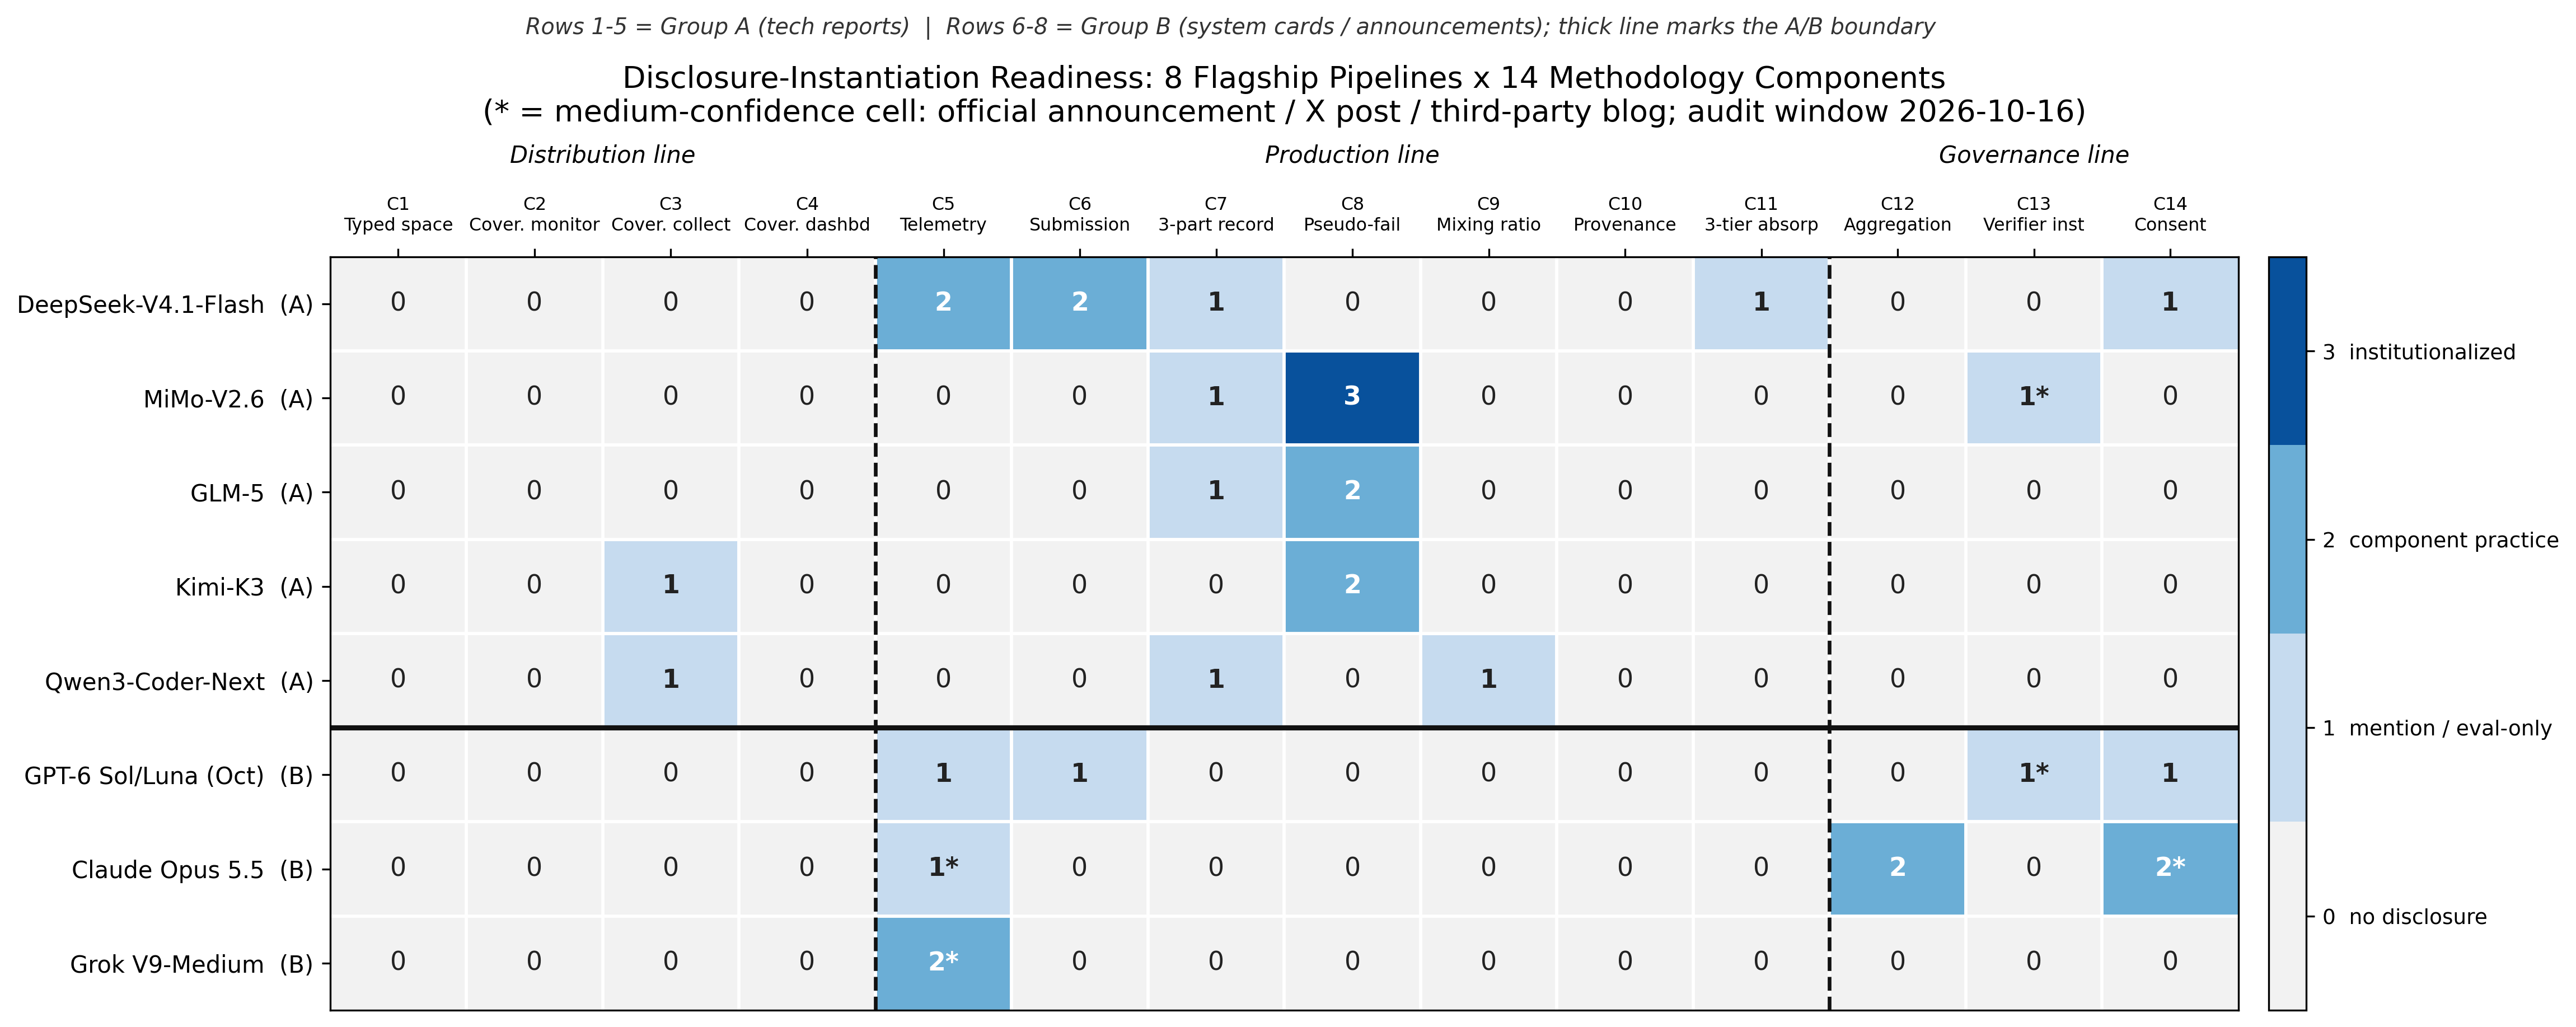
\includegraphics[width=\textwidth]{figures/fig2_readiness_heatmap.png}
\caption{Disclosure-instantiation readiness. Levels 0--3 for 8 flagship pipelines $\times$ 14 components (rows 1--5 = Group A tech reports; rows 6--8 = Group B system cards/announcements; thick line = A/B boundary; dashed lines = methodology-line boundaries; * = medium-confidence cell). The empty band across C1/C2/C4/C10 and the absence of any level-2 cell in C7 are visible at a glance.}
\label{fig:heatmap}
\end{figure}

\textbf{Headline readings.} The matrix totals 32 of 112 possible points (mean level 0.286). Eighty-nine cells (79.5\%) are zero; 23 cells (20.5\%) are non-zero, of which 15 are level 1 (13.4\% of all cells), 7 level 2 (6.2\%), and exactly one level 3 (0.9\%) --- MiMo-V2.6 on pseudo-failure discrimination (89 + 23 = 112; level percentages are computed against all 112 cells and rounded to one decimal). Four components are absent from every disclosure: typed space (C1), coverage monitor (C2), coverage dashboard (C4), and provenance stratification (C10). Three-part failure records peak at level 1: the two components of the record that exist in disclosures (recognizable error, explicit correction) have not been joined anywhere by the third (root cause) or by a packaging protocol --- the audit's precise location of the vacancy. The closest pipeline to the methodology is DeepSeek-V4.1-Flash (7 points, mean 0.500), with the most complete production-side picture (collection at C5/C6 both level 2, plus replay fragments); the single deepest cell belongs to MiMo-V2.6. The three lines separate sharply: production 0.393, governance 0.333, distribution 0.062. Two structural facts refine the separation. First, governance-line instantiation is a single-laboratory phenomenon: Group B's governance mean of 0.667 is contributed almost entirely by one pipeline; excluding it, the governance line's remaining 21 cells hold 4 points, an industry-wide governance mean of 0.190. Governance instantiation is therefore concentrated rather than widespread. Second, Group A's scores cluster in the production-cleaning segment (C5--C8) while Group B's lone contributor scores on the governance line --- the audit set's variance is structural, not random.

Reading the levels. A level-2 cell names a mechanism that can be pointed at: who submits, how environments are sanitized, which corpus is synthetic. A level-3 cell adds an institutional marker --- a quantity, a platform figure, a governance document, or independent audit --- and exactly one cell in the set meets that bar. The pattern across Tables~\ref{tab:matrix} and \ref{tab:components} is therefore not that flagship pipelines lack engineering, but that their engineering is disclosed as narrative rather than as institution: mechanisms without quantities (capped at 2 by rule) and evaluation-side uses that never cross into training (capped at 1 by rule). The audit instrument was built to see precisely this difference; the readiness gap is made of it.

\subsection{Sensitivity}

Excluding all five medium-confidence cells (no low-confidence cells exist) --- MiMo$\times$C13 and GPT-6$\times$C13 (third-party-audit disclosures), Opus$\times$C5 and Opus$\times$C14 (system-card statements), and Grok$\times$C5 (CEO announcement posts) --- leaves 25 points (mean 0.223): the four all-zero components remain all-zero, C7's maximum remains 1 (its evidence is all high-confidence), the three-line ordering is unchanged, and the single level-3 cell stands. What the medium filter does remove is the two load-bearing ones among them --- Grok's real-workflow case and Opus's consent cell --- which is why Grok is cited throughout this paper only with its announcement-level qualifier: under a high-confidence-only reading, the strongest public signal that real developer workflows are entering supplementary training rests on two posts \cite{ref21}. A construct-strictness check on C3: its two level-1 cells are near-constructs (underrepresented-knowledge retrieval; task-diversity scaling), so under the strict typed-coverage definition C3 is 0/8. The gap claim of Section 3 holds under both counts; we report and rely on the strict one.

\subsection{What the audit does not establish}

Four limits, stated to prevent the descriptive section from leaking into the normative ones. (i) The construct is disclosure: a laboratory may implement typed coverage silently; the audit measures the public interface of practice. (ii) Table~\ref{tab:lines} is \emph{not} a verification of any claim about governance lagging engineering in the literature: that comparison tracks how institutional mechanisms lag research output over time, whereas the matrix measures flagship-pipeline instantiation at one date --- different constructs; the only governance claim the matrix supports is its own (verifier institutionalization, C13, peaks at level 1 in this set). (iii) The distribution line's empty band is a fact about disclosure in this set, not a proof that coverage-driven collection would improve any pipeline --- that is Section 3's normative argument, which stands on theory and literature. (iv) Three evidence notes: the misalignment-reporting portal showed 19 reports on 2026-10-16 (earlier secondary counts of 6 are superseded); a ``failure-mode tracking'' keyword attributed to one pipeline's report was not confirmed in its full text (its confirmed disclosure, a hacking-detection system, is coded under C8); and one pending cell (Claude Opus 5.5 $\times$ C8) awaits location of a referenced audit document --- if found and it matches, the affected line totals rise by at most 2 points, changing no conclusion above.

\section{Translation: One Methodology, Four Audiences}

A methodology that cannot cross into the dialects of the communities that would implement it remains a manuscript. This section offers four bridges. The discourse evidence is illustrative, not representative: each community is heterogeneous, and the bridges rest on design arguments plus the cited texts. All four communities have one thing in common, and it is the opening every bridge exploits: each has reached the edge of dynamic data in its own vocabulary --- rollouts, dumps, consent, mirrors --- and each, by default, takes the \emph{experiencing subject} to be the agent. The era-of-experience essay itself leaves the door open: ``a small amount of human data may facilitate a large amount of autonomous learning'' \cite{ref3}. The methodology flips the subject back: the stream that matters is the human one.

\subsection{Agent-RL practitioners}

\emph{Bridge vocabulary.} rollout, trajectory, environment, staleness $\leftrightarrow$ practice-flow telemetry; the entry phrase is \textbf{the human side of on-policy rollouts}. The community already treats behavior as a perpetual data stream --- its infrastructure (sandbox fleets, replay buffers, staleness controllers \cite{ref48,ref49}) is the production line of Section 4 with one subject swapped. \emph{Pains mapped to concepts.} Reward hacking $\to$ failure attribution data (C7/C8): the difference between a true failure and a gamed reward is exactly the root-cause record. Entropy and solution-mode collapse \cite{ref11} $\to$ the injection rate (C9): fresh human practice is the external entropy source. Evaluation drift $\to$ the fitting lag (C11): offline evals and deployment diverge on the same clock the staleness metric already measures. \emph{Objections and replies.} (a) ``Human data is dirty and expensive.'' Failure cases are the cheap slice --- organizations already pay to collect them (bounty programs; employee workflows \cite{ref20}), and the expensive part (attribution) is the part RL systems need anyway. (b) ``Synthetic and self-play suffice.'' In verifiable domains, largely yes --- Section 4.5 concedes this and builds the domain split into the protocol; what no compiler verifies is whether a value, a workflow habit, or a novice's misconception is real. (c) ``We do RLVR, not imitation.'' The verifier is a human institution: the frontier community's own summaries put it as a check you can execute rather than a model of preferences \cite{ref66} --- and checks encode human decisions, which drift as practice drifts. The sharpest ally here is a critic of the experience narrative, who writes that for humans and human-like systems ``we should be talking about `training environments', not `training data''' \cite{ref67} --- the methodology's production line is precisely the governance of training environments \emph{and} the data they emit.

\subsection{Pre-training and data engineers}

\emph{Bridge vocabulary.} dump, snapshot, dedup, mixture, contamination $\leftrightarrow$ typed incremental corpus; the entry phrase is \textbf{the never-finalized, time-incremental corpus}. The community's pains are the stock-flow mismatch in disguise: the web is a stream and the corpus is a snapshot, so the wall \cite{ref1}, the staleness, and the contamination are one problem. \emph{Pains mapped to concepts.} Wall $\to$ restate as: only the stock is walled; the flow of practice (issues, corrections, workflows, feedback) never stops. Mixtures as art $\to$ C9's domain-typed floors. Contamination $\to$ C10's provenance strata; once watermarks survive training \cite{ref44}, AI-mediated text becomes a measurable stratum rather than an invisible one. Cadence $\to$ C11 and time-incremental CPT \cite{ref47}. \emph{Objections and replies.} (a) ``We already do CPT and mid-training mixes.'' Cadence without typed coverage leaves the distribution line at zero --- Section 6's C1/C2/C4 columns are what that looks like from outside. (b) ``Flywheels are already industry practice.'' Data flywheels exist as engineering narratives --- one observability company has published its 9B alert-investigation model trained on curated internal workflow data \cite{ref8} --- but as fragments: no typed schema, no failure records, no per-domain floors, no verification ladder. The methodology is the assembly, not the invention. (c) ``Fresh data breaks reproducibility.'' Versioned schemas (C1) and archived dashboards (C4) exist to make the flow auditable; a frozen corpus is reproducible the way a fossil is.

\subsection{Governance and policy}

\emph{Bridge vocabulary.} provenance, consent, licensing, training-data summary $\leftrightarrow$ feasible-set registry; the entry phrase is \textbf{consent as a continuing relationship}. The community already holds the needed legal concept --- consent that is revocable and context-dependent under the GDPR \cite{ref60} --- and has documented what one-shot collection does to it: ``dubious collection practices have spurred crises in data transparency, consent, and provenance'' \cite{ref9}. \emph{Pains mapped to concepts.} Untraceable consent $\to$ C14's machine-readable terms \cite{ref59}; the buyout economy's instability \cite{ref10,ref63} $\to$ flow licensing priced on duration and revocation; the AI Office's summary regime \cite{ref17} $\to$ C4 dashboards as the indicator-level counterpart to content summaries. \emph{Objections and replies.} (a) ``Privacy law forbids this scale of collection.'' The feasible set is a boundary condition of the methodology, not an objection to it: C14 exists to make the constraint computable --- 30-day windows, opt-in defaults, sharded retraining on withdrawal \cite{ref61} are all pipeline components already. (b) ``It advantages large platforms.'' The typed schema and the consent protocol are the two components a small actor can adopt unilaterally; asymmetric flywheels are the alternative's status quo. (c) ``Provenance cannot be enforced.'' Watermark deployment under the EU regime \cite{ref42} and origin-enforced consent protocols are the first enforcement-grade primitives.

\subsection{Philosophy and public discourse}

\emph{Bridge vocabulary.} mirror, snapshot of culture, frozen past $\leftrightarrow$ \textbf{the living mirror}. The philosophical critique of current models is that they freeze a moment: ``The image of our data that appears in the AI mirror can be dim or blurred or fogged or distorted, but it cannot be unknown, unmade'' \cite{ref68}. The methodology's answer is not a better polish but a moving surface: a practice-fitted system reflects what people are doing, including failing and learning --- and because the fitting object is practice rather than works, attribution, change, and refusal travel with the data (C14) instead of being stripped at ingestion. \emph{Pains mapped to concepts.} Frozen self-image $\to$ C11's fitting lag made public (staleness as an honest label); dehumanizing idealization $\to$ the typed schema's outcome and expertise axes, which guarantee that novices' failures and experts' corrections enter the record, against any corpus of polished artifacts; extraction without voice $\to$ aggregation with declared rules (C12). \emph{Objections and replies.} (a) ``You are reifying humans into data.'' The typing includes failure and typicality by design --- the opposite of an idealized portrait; and the feasible set keeps the description revocable. (b) ``This makes the mirror more persuasive, hence more dangerous.'' Persuasiveness tracks accuracy of reflection; a mirror that admits staleness and coverage gaps is more corrigible than one that implies completeness. (c) ``Whose practice counts?'' --- exactly the question C12 forces into a written, revisable rule, which is more than a silent aggregation function offers.

\section{Metrics and Falsification}

\subsection{The methodology dashboard}

Five indicators, one per line plus two cross-cutting, each with a falsifiable target: (1) \textbf{cell coverage} --- $\Sigma\,\min(\hat{q},\hat{p})$ over typed cells, with empty-cell count and smallest-cell alarms (C2/C4); (2) \textbf{fitting lag} --- per-layer median time from data generation to absorption, reported with the snapshot cycle $\Delta$ (C11); (3) \textbf{injection rate} --- the effective share of freshly collected human practice per domain, reported against C9's floors, with the domain split (verifiable / semi-verifiable / open) stated; (4) \textbf{pseudo-failure discrimination rate} --- the share of submitted ``failures'' reclassified as environment-caused or gamed before training, plus replay-pass rate of corrections (C7/C8); (5) \textbf{readiness score} --- the audit's mean level for a pipeline or ecosystem, recomputed on the frozen scale as disclosures evolve (Section 6). A dashboard convention from the memory-systems literature applies to all five: a number without a stated method is a claim, not a result \cite{ref50}.

\subsection{Falsification conditions}

The methodology is stated so that evidence can kill its parts. \textbf{Distribution line.} If quota-based representativeness is shown to outperform typed coverage-driven collection in a production pipeline (on joint-distribution metrics, not marginals), Section 3 is rebuilt. If coverage monitoring proves unrelated to downstream robustness under distribution shift, C2/C4 demote to bookkeeping. If typed operationalization of experience coverage becomes common in training-objective specifications, the gap claim of Section 3.1 fails. \textbf{Production line.} If an open-domain pipeline sustains training on a purely synthetic stream without collapse \emph{and} without a human-pretrained base, the injection-rate design of C9 fails at its root. If three-part failure records prove no better than paired failure-success data on transfer metrics, C7 demotes to a formatting convention. If deployment-time online weight absorption becomes standard practice with lag controlled, C11's three-tier premise is obsolete. \textbf{Governance line.} If flagship disclosures show the three lines institutionalized (level-3 cells across C1, C9, C13), this paper's readiness findings reduce to a dated confirmation, and the methodology's prescriptive content transfers to maintenance. The one falsification that has already occurred --- verifiable-domain synthetic self-sufficiency (AZR \cite{ref37}, Ring-Zero \cite{ref38}, and the synthetic-corpus scaling results \cite{ref36}) --- was absorbed as a design parameter in Section 4.5 rather than denied: the domain split \emph{is} the revised claim. Current empirical baseline for every condition: Section 6, Table~\ref{tab:matrix}.

\section{Conclusion}

The human-referential fitting theory's temporal clause has an engineering reading, and this paper has tried to write it out in full. If the object of fitting is human practice --- the full spectrum of who succeeds, who fails, who is learning --- and the full course over which practice unfolds, then no frozen corpus can carry it, and no purely synthetic recursion can correct it in the domains where correction matters most. Something must stand between the living practice and the learning weights: a stack that types what it collects (C1--C4), never stops collecting and never stops cleaning (C5--C11), and answers --- in writing, under audit --- whose practice it fits, who adjudicates its failures, and what may still be withdrawn (C12--C14). The readiness audit says the pieces exist in isolation, sometimes at depth (one pipeline holds a level-3 cell in pseudo-failure discrimination), while the distribution line sits at 0.062 and four components are disclosed nowhere. The distance between the protocol and the disclosure record is the work program. \textbf{The stock has a wall; the flow does not --- and the flow requires a stack.} What the audit adds to the clause is a measuring rod for the stack's arrival.

The methodology points to its own next steps. On the normative side: reference implementations of the typed schema and the coverage monitor over an open failure-case corpus --- the most actionable validation of the component pair doubly absent from literature and disclosure. On the audit side: the inter-rater blind recoding and data freeze proceed under the protocol of Section 6.1, and the readiness score will be recomputed on the frozen scale as disclosures evolve (Section 8.1).

\section*{Data and Code Availability}

The audit matrix (112 cells with levels, confidence grades, verbatim quotes, and locators), the full quote archive, and all figure- and table-generation scripts are archived in the project workspace; a public release of the audit materials will accompany the publication decision.

\section*{Author Contributions and Disclosures}

Single author (Y.Y.): conceptualization, methodology, audit coding, analysis, and writing. No funding was received for this work. The author declares no conflicts of interest. The study is a public-document audit involving no human subjects. This manuscript was prepared with AI-assisted drafting and literature-retrieval tooling under the direction of the author, who verified all primary sources and takes full responsibility for the content. The work builds on two independently published companion works, cited here as \cite{ref5} and \cite{ref6}.

\bibliographystyle{unsrtnat}
\bibliography{references}

\end{document}
